%%%%%%%%%%%%%%%%%%%%%%%%%%%%%%%%%%%%%%%%%%%%%%%%%%%%%%%%%%%%%%%%%%%%%%%%%%%%%%%
%
% witseiepaper-2005.tex
%
%                       Ken Nixon (12 October 2005)
%
%                       Sample Paper for ELEN417/455 2005
%
%%%%%%%%%%%%%%%%%%%%%%%%%%%%%%%%%%%%%%%%%%%%%%%%%%%%%%%%%%%%%%%%%%%%%%%%%%%%%%%%

\documentclass[10pt,twocolumn]{witseiepaper}

%
% All KJN's macros and goodies (some shameless borrowing from SPL)
\usepackage{KJN}
\usepackage{xcolor}
\usepackage{graphicx}
\usepackage[table,xcdraw]{xcolor}
\usepackage{multirow}
\usepackage{multicol}
\usepackage{tabularx,ragged2e}
%
% PDF Info
%
\ifpdf
\pdfinfo{
/Title (INSTRUCTIONS AND STYLE GUIDELINES FOR THE PREPARATION OF FINAL YEAR LABORATORY PROJECT PAPERS : 2005 VERSION)
/Author (Ken J Nixon)
/CreationDate (D:200309251200)
/ModDate (D:200510121530)
/Subject (ELEN417/455 Paper Format, 2005)
/Keywords (ELEN417, ELEN455, paper, instructions, style guidelines, laboratory project)
}
\fi

%%%%%%%%%%%%%%%%%%%%%%%%%%%%%%%%%%%%%%%%%%%%%%%%%%%%%%%%%%%%%%%%%%%%%%%%%%%%%%%
\begin{document}


%\title{DESIGN AND IMPLEMENTATION OF A HEARTBEAT SEGMENTATION AND CLASSIFICATION MODEL}
\title{Project Plan for the Design and Implementation of a Heartbeat Segmentation and Classification Model}

\author{Boikanyo Radiokana (1386807) \\ Elias Sepuru (1427726) \\ Group: 19G11 \\Supervisor: Ellen de Mello Koch
\thanks{School of Electrical \& Information Engineering, University of the
Witwatersrand, Private Bag 3, 2050, Johannesburg, South Africa}
}


%%%%%%%%%%%%%%%%%%%%%%%%%%%%%%%%%%%%%%%%%%%%%%%%%%%%%%%%%%%%%%%%%%%%%%%%%%%%%%%
%
\abstract{This paper presents a  plan  to  design and implement  a  Heartbeat  Segmentation and Classification Model.  The
model is divided into 3 main sections namely: Preprocessing, Segmentation and Classification.  The preprocessing  stage involves  reducing  noise  from  the  hearbeat signals and conditioning it for segmentation. The signal will be downsampled with a factor ranging from 10 - 20. Segmentation will be performed by computing the signals average Shannon energy. Classification is to be be implemented with machine learning methods such as ANN and RNN. Project management concepts such as work-division and risk management are also taken into consideration.}

\keywords{Classification, Noise, Preprocessing, Segmentation}


\maketitle
\thispagestyle{empty}\pagestyle{empty}


%%%%%%%%%%%%%%%%%%%%%%%%%%%%%%%%%%%%%%%%%%%%%%%%%%%%%%%%%%%%%%%%%%%%%%%%%%%%%%%
%
\section{INTRODUCTION}
Cardiovascular diseases (CVDs) continue to be one of the leading causes of deaths around the world. More people die annually from CVDs than  any other cause. In 2016 alone an estimated 31\% of the deaths were due to CVDs \cite{WHO}. Methods to detect early signs of heart diseases could prove to be very helpful in preventing deaths due to CVDs. 

This paper presents the plan of Heartbeat Segmentation and Classification project. The project aims to create a first level screening for individuals in the detection of heart diseases. This will aid medical practitioners in their field and possibly home use by individuals.

In the upcoming sections, the background, system overview, design methodology and project management are discussed.

\section{BACKGROUND}
\subsection{Project Specifications and Requirements}
\label{PSR}
The aim of this project is to create a first level screening to detect signs of heart diseases in individuals. This will be carried out by using audio data sets from two sources, the iStethoscope Pro iPhone app labelled Dataset A and a digital stethoscope labelled Dataset B. The audio data was recorded by the general public and clinical healthcare practitioners respectively \cite{pascal}. Both data sets A and B each have different categories which all contain various background noises. The audio files vary in length from 1 to 30 seconds as a means of reducing excessive noise \cite{pascal}. Dataset A is said to consist of the the following categories, namely; Normal, Murmur, Extra Heart Sound and Artifact whilst Dataset B has Normal, Murmur and Extrasystole categories. The above mentioned categories will be used as classifiers at a later stage.

With the excessive noise present in the audio data, it is required that preprocessing methods, capable of removing noise from the data be implemented before execution of further detection methods. Following the denoising process, a method to locate S1 (lub) and S2 (dub) heart sounds as well as segmentation of Normal audio files from the two data sets is required. A machine learning method to classify heartbeat sounds into normal and diseased categories as mentioned above must be implemented.

%%%%%%%%%%%%%%%%%%%%%%%%%%%%%%%%%%%%%%%%%%%%%%%%%%%%%%%%%%%%%%

%%%%%%%%%%%%%%%%%
\subsection{Assumptions}
The project is to be conducted with the following assumptions:

\begin{itemize}
    \item The audio data range will be 30 seconds and less.
    \item Dataset A has only four categories (Normal, Murmur, Extra heart sound and Artifacts) and Dataset B has only three categories (Normal, Murmur and Extrasystole)
\end{itemize}

\subsection{Constrains}
The following are the project constraints:

\begin{itemize}
    \item Constrained to only locating S1 (lub) and S2 (dub) heart sounds
    \item Only the Normal audio data is to be used for the location of S1 and S2.
    \item Only the data from here {\url{https://www.kaggle.com/kinguistics/heartbeat-sounds/kernels}} can be used, due to ethics clearance
    \item Heart sounds are only in \texttt{.wav} and \texttt{.aif} format
\end{itemize}
\subsection{Success Criteria}
For the project to be deemed successful it has to meet all the requirements specified in section \ref{PSR}. Since existing solution only have an accuracy of up to 77\%, an accuracy of 77\% or higher is highly desirable.

%%%%%%%%%%%%%%%%%%%%%%%%%%%%%%%%%%%%%%%%%%%%%%%%%%%%%%%%%%%%%%%%%%%%%%%%%%%%%%%
\subsection{Literature Review}
Cardiovascular diseases continue to be one of the leading cause of deaths around the world \cite{WHO}.  With the above mentioned there have been various attempts to accurately distinguish between normal and diseased heartbeat sounds using ECG and PCG.  Groch uses a microprocessor controlled Heart-Sound Gate (HSG), which automatically identifies heart sounds from PCG alone, using timing relationships \cite{groch1992new}. He amplifies the heart sound and passes it through two bandpass filters, folds the negative portions of the waveform into the positive and the envelopes the whole signal. To locate the peaks he uses a Schmitt trigger which then generates a square wave corresponding to the peaks. To identify S1 and S2, he exploits the fact that the diastolic period is longer than the systolic period. 

Karraz \textit{et al.} makes use of data from MIT-BIH Arrhythmia database, to classify the heartbeats into five categories. They use an FIR filter set at (0.05 - 40 Hz) cut-off and a notch filter for denoising the signals, for peak location and S1 and S2 identification they use a QRS detection algorithm. To classify the heartbeat sounds into the different categories they picked, they use the Bayesian Artificial Neural Network (BANN) with the following features: i) P-amplitude, ii) P-wide, iii)R-amplitude, iv) Q-amplitude, v) S-amplitude, vi) QRS-wide, vii)T-amplitude, viii) T-wide, ix) PR-period, and x) RR-period \cite{karraz2006automatic}. Kampouri  also uses the QRS complex for feature extraction but instead of Neural Networks, he uses Support Vector Machine (SVM) \cite{kampouraki2008heartbeat}.


Stunic \textit{et al.} detects and classifies heart murmurs using segmentation techniques and ANN. This study is conducted using simulated and recorded patient heart sounds. The segmentation algorithm identifies individual heart cycles and an average of all cycles is computed to extract components within 195Hz since this band has the most valuable information \cite{strunic}. The basis of the segmentation algorithm is the fact that the diastolic period is longer than the systolic period. They used an alignment algorithm to ensure that data is always fed in the same order to the ANN input neurons. The ANN algorithm consists of 3 hidden layers with 25 input neurons each and 1 output neuron. The diagnostic system presented an accuracy of 48,7$\pm$12,7\% for real life recorded patient records and an accuracy of 85$\pm$7,4\% for simulated data \cite{strunic}.

To combat the issues of noise in real life recordings of heartbeat sounds Liang \textit{et al.} uses a Chebyshev type I lowpass filter and an algorithm  based on the normalised average Shannon energy of a PCG signal. The algorithm is used to find the peak locations and to pick up the locations of S1 and S2. It achieves 93\% correct ratio \cite{liang1997heart}. Debbal \textit{et al.} uses Discrete Wavelet Transform (DWT) to decompose and reconstruct a PCG signal with insignificant loss of information. The error found in reconstructing the signal is considered as an important feature in the classification of diseased categories. It was found that the reconstruction error increases with an increase in murmur intensity \cite{debbal}.


%%%%%%%%%%%%%%%%%%%%%%%%%%%%%%%%%%%%%%%%%%%%%%%%%%%%%%%%%%%%%%%%%%%%%%%%%%%%%%%

\section{SYSTEM OVERVIEW}

\begin{figure}[h!]
    \centering
    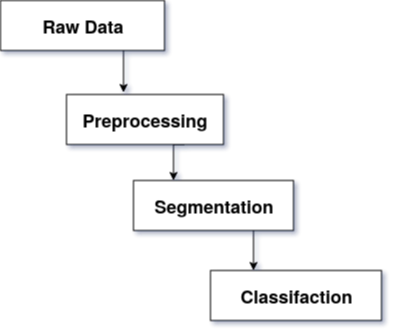
\includegraphics[scale = 0.7]{systemOverviw.png}
    \caption{System Overview}
    \label{fig:sysov}
\end{figure}{}


Figure \ref{fig:sysov} above illustrates an overview of the proposed system. The raw data is read from the two datasets, Dataset A and Dataset B as mentioned in the section \ref{PSR}. The audio data can either be in \texttt{.wav} or \texttt{.aif} format.
As mentioned previously, the audio data sets contain excessive noise which requires denoising before segmentation can take place. This denoisong process is performed in the preprocessing phase to ensure that the data is conditioned for segmentation. Once the data is conditioned, it goes through the segmentation phase where S1 and S2 are located. This is done in order to extract important features useful for classification. The features will be fed into a machine learning algorithm in order to classify the heart sounds into normal or diseased categories.

%%%%%%%%%%%%%%%%%%%%%%%%%%%%%%%%%%%%%%%%%%%%%%%%%%%%%%%%%%%%%%%%%%%%%%%%%%%%%%%
%
\section{DESIGN METHODOLOGY}

The project in its entirety mainly consists of two main sections, heartbeat segmentation and heartbeat classification. However, due to the fact that data cleansing forms the bulk of the project, it was decided that it will be suitable to make preprocessing a standalone section as seen in figure \ref{fig:sysov}. This will also help break down the project into manageable tasks.

\subsection{Preprocessing}
As mentioned earlier the audio data is from real world situations and contains a lot of background noise, in the processing phase, techniques to remove the background noise are applied to the audio data.

The audio data has a sampling frequency of 44.1 kHz. The first stage of denoising the signal involves downsampling the signal with a factor between 10 - 20. Since it is known that the highest desired frequency is that of the murmur which is 600 Hz \cite{mumur}, downsampling by the highest factor, which is 20, will still give a sampling frequency higher than twice that of a murmur. Downsampling helps with cutting high frequency components, exploiting the Nyquist Theorem. The high frequency components are aliased whilst preserving the desired low frequency components. Downsampling also compresses the size of the audio data, allowing for faster processing time \cite{lavry2004sampling}.

Most of the information of a PCG signal is contained in the lower frequency components of the signal as mentioned in the above paragraph. With that mentioned a low pass filter of 195 Hz will be applied after downsampling to further curb the noise \cite{pascal}.

The final stage of preprocessing involves normalising the signal to the absolute maximum of the signal using equation \ref{eq:1} \cite{liang1997heart}.

\begin{equation}
    x_{norm}(i) = \frac{x_{f_{ds}}(i)}{max_{j}(|x_{f_{ds}}(j)|)}
    \label{eq:1}
\end{equation}{}
where $x_{f_{ds}}$ is the downsampled signal. 
Figure \ref{fig:pre} summarises the preprocessing phase.

\begin{figure}[h!]
    \centering
    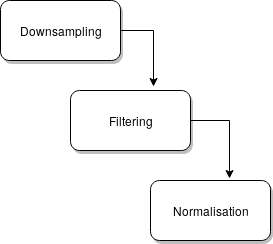
\includegraphics[scale=0.7]{Project_Plan/preproc.png}
    \caption{Flow diagram of the preprocessing phase}
    \label{fig:pre}
\end{figure}{}

\subsection{Heartbeat Segmentation}
The segmentation phase involves locating S1 and S2 heart sounds, thus determining the diastolic and systolic periods. To segment these heart sounds, the envelope of the normalized signal obtained in the preprocessing phase is computed. The Shannon energy will be used to compute the envelope of the signal with equation \cite{liang1997heart}:

\begin{equation}
    E = -x^2log(x^2)
\end{equation}{}

The reason for choosing this method is the fact that Shannon energy attenuates small spikes in signals much more than large spikes \cite{liang1997heart}. Furthermore, a triangular smooth function will be applied to smoothen out the signal since the signal will still contain small spikes. Equation 3 below will then be used to determine the average Shannon energy of the entire signal \cite{liang1997heart}:

\begin{equation}
    E_s = -\frac{1}{N}\sum_{i=1}^{N} x_{norm}^{2}(i)logx_{norm}^{2}(i)
\end{equation}{}
 where \(x_{norm}\) is the value of the normalized sample signal and \(N\) is the signal length. This is followed by the computation of the normalized average Shannon energy using equation 4 below \cite{liang1997heart}:
 
 \begin{equation}
     P_a(t) = \frac{E_s(t)-M(E_s(t))}{S(E_s(t))}
 \end{equation}{}
 
 where \(M(E_s(t))\) is the mean of \(E_s(t)\) and \(S(E_s(t))\) is the standard deviation of \(E_s(t)\).
 
 \subsubsection{Peak Identification}
\textcolor{white}{B} \\ 
 The peaks representing the heart sounds S1 and S2 will be identified with a function in Matlab called peakdet \cite{gomes2012classifying}. One advantage of using this function is that it is an open source function and therefore allows one to condition it to best suite their needs. S1 and S2 will be located by exploiting the fact that diastolic period is greater than systolic period.
 
\subsection{Heartbeat Classification}
The classification phase involves coming up with a model, given a specific audio file, will successfully identify it as either one of the categories in Dataset A or one of the categories in Dataset B. Before training the model, feature construction and selection has to occur first. The features are to be constructed from the locations of S1 and S2.

Table \ref{tab:features} presents the possible features that could be used to train the machine learning models \cite{gomes2012classifying}.

\begin{table}[h!]
\centering
\caption{Potential feature selection}
\label{tab:features}
\begin{tabular}{|l|l|}
\hline
\textbf{Feature} & \multicolumn{1}{c|}{\textbf{Description}} \\ \hline
N & Number of heartbeats per minute \\ \hline
M_{1} & Mean of diastole period \\ \hline
M_{2} & Mean of systole period \\ \hline
R_{s1} & \begin{tabular}[c]{@{}l@{}}Standard deviation of S1 over \\ the standard deviation of the\\ whole signal\end{tabular} \\ \hline
R_{s2} & \begin{tabular}[c]{@{}l@{}}Standard deviation of S2 over \\ the standard deviation of the\\ whole signal\end{tabular} \\ \hline
R_{m1} & \begin{tabular}[c]{@{}l@{}}Mean of S1 over the total mean\\ of the entire signal\end{tabular} \\ \hline
R_{m2} & \begin{tabular}[c]{@{}l@{}}Mean of S2 over the total mean\\ of the entire signal\end{tabular} \\ \hline
R_{med} & \begin{tabular}[c]{@{}l@{}}Ratio of the median of the three\\ largest segments in the sample\\ over the total mean\end{tabular} \\ \hline
R_{sq} & \begin{tabular}[c]{@{}l@{}}Square of the array of the sorted\\ segments of the sample\end{tabular} \\ \hline
\end{tabular}
\end{table}

The features shown in table \ref{tab:features} are to be carefully selected in order to cater and distinguish for the different categories in Dataset A and Dataset B.

For training, two models, ANN and RNN are chosen. ANN is chosen due to its good ability to recognise patterns \cite{demuth2014neural}. The RNN is also chosen for its great pattern recognition and its ability to handle many-to-many predictions problems \cite{he2019automatic}.
%\newpage
\section{TESTING}
In order to allow for testing the machine learning algorithms will be trained according to 7:3 ratio. This means that 70\% of the audio data will be used for training whilst the other 30\% will be for testing to generate the F-score, Youden’s Index and the Discriminant Power.

%%%%%%%%%%%%%%%%%%%%%%%%%%%%%%%%%%%%%%%%%%%%%%%%%%%%%%%%%%%%%%%%%%%%%%%%%%%%%%%
%


% Please add the following required packages to your document preamble:

\section{PROJECT MANAGEMENT}

\subsection{Work Division}
The project will be conducted by a team of two people. Each section in the project as illustrated in figure \ref{fig:sysov}
will be allocated two different techniques. Each team member will then be assigned a technique to follow to solve a particular section. The technique that yields the best accuracy will be the approach chosen for the project. Table \ref{work-div} below shows a detailed work division amongst the members of the team.


% Please add the following required packages to your document preamble:
% \usepackage{multirow}
\begin{table}[h!]
\centering
\caption{Work Division}
\label{work-div}
\begin{tabular}{|l|c|l|}
\hline
\textbf{Task} & \multicolumn{1}{l|}{\textbf{Technique}} & \textbf{\begin{tabular}[c]{@{}l@{}}Team \\ Member\end{tabular}} \\ \hline
\begin{tabular}[c]{@{}l@{}}Environment\\ Setup\end{tabular} & - & Both \\ \hline
\multirow{2}{*}{Preprocessing} & 1 & Elias \\ \cline{2-3} 
 & 2 & Boikanyo \\ \hline
\multirow{2}{*}{Segmentation} & 1 & Elias \\ \cline{2-3} 
 & 2 & Boikanyo \\ \hline
\multirow{2}{*}{\begin{tabular}[c]{@{}l@{}}Classification, Training \\ and Testing\end{tabular}} & 1 & Elias \\ \cline{2-3} 
 & 2 & Boikanyo \\ \hline
Documetation & - & Both \\ \hline
\end{tabular}
\end{table}
%%%%%%%%%%%%%%%%%%%%%%%%%%%%%%%%%%%%%%%%%%%%%%%%%%%%%%%%%%%%%%%%%%%
\subsection{Project Time-line}
The project will officially be started on the $15^{th}$ July 2019 following extensive research by both team members. The project deadline is on the $6^{th}$ September 2019. All in all the project is said to run for six weeks. Table \ref{tab:my-table} shows all the project milestones and completion dates.

\begin{table}[h!]
\centering
\caption{Project Milestone Completion}
\label{tab:my-table}
\begin{tabular}{|c|c|}
\hline
\textbf{Completion Date} & \textbf{Milestone} \\ \hline
15 July 2019 & Project  Planning \\ \hline
16 July 2019 & Environment Setup \\ \hline
31 July 2019 & Data Cleansing \\ \hline
09 Aug 2019 & Segmentation \\ \hline
30 Aug 2019 & \begin{tabular}[c]{@{}c@{}}Classification(Model Training \\ and Testing)\end{tabular} \\ \hline
06 Sep 2019 & \begin{tabular}[c]{@{}c@{}}Documentation (Final Project\\ Report)\end{tabular} \\ \hline
\end{tabular}
\end{table}

%%%%%%%%%%%%%%%%%%%%%%%%%%%%%%%%%%%%%%%%%%%%%%%%%%%%%%%%%%%%%%%%%%%%%
\subsection{Resource Management}
The following resources (hardware and software) will be necessary to successfully carry out the project:

\begin{itemize}
    \item Two compatible computers for data
cleansing, training and testing of the
models
\item Clusters for processing big data
  \item MATLAB and Jupyter Notebook for
signal processing and building models
\item KNIME and Anaconda building models
\item Internet for research
\item Digital Stethoscope.
\item Funds for printing of technical report and
the poster for open day.
\end{itemize}{}

%%%%%%%%%%%%%%%%%%%%%%%%%%%%%%%%%%%%%%%%%%%%%%%%%%%%%%%%%%%%%%%%%%%%%
\subsection{Risk Management}

Potential risks that can possibly jeopardise the success of the project have been identified. The risk register in table \ref{risk-register} shows the cause of each risk that is identified, its rating, degree of impact as well as the action that should be taken to mitigate the risk.


\begin{table*}[h!]
\centering
\caption{Project Risk Register}
\label{risk-register}
\resizebox{\textwidth}{!}{%
\begin{tabular}{|l|l|c|c|l|l|}
\hline
\textbf{Risk} & \textbf{Cause} & \textbf{Risk Rating} & \textbf{Impact} & \textbf{Actions} & \textbf{\begin{tabular}[c]{@{}l@{}}Person \\ Responsible\end{tabular}} \\ \hline
Machines crashing & \begin{tabular}[c]{@{}l@{}}Software installation \\ and Processing Big \\ data\end{tabular} & H & H & \begin{tabular}[c]{@{}l@{}}Use clusters provided by \\ Professor Otto for running \\ big data simulations and proper\\ software installations\end{tabular} & Both members \\ \hline
\begin{tabular}[c]{@{}l@{}}Failure to remove \\ noise\end{tabular} & \begin{tabular}[c]{@{}l@{}}Application of \\ incorrect techniques\end{tabular} & H & H & \begin{tabular}[c]{@{}l@{}}Use of alternative secondary \\ open-source data from MIT. Use\\  of predefined methods\end{tabular} & Both members \\ \hline
Mislocation of S1 and S2 & \begin{tabular}[c]{@{}l@{}}Using incorrect \\ techniques\end{tabular} & M & M & \begin{tabular}[c]{@{}l@{}}Use of multiple methods of locating \\ S1 and S2 to check for any errors \\ and correspondence of the results.\end{tabular} & Both members \\ \hline
Loss of work & \begin{tabular}[c]{@{}l@{}}Not saving copies\\ of completed work\end{tabular} & H & H & \begin{tabular}[c]{@{}l@{}}Use Github for version\\ control\end{tabular} & Both members \\ \hline
\begin{tabular}[c]{@{}l@{}}Poor milestone \\ estimation and project\\ running behind schedule\end{tabular} & \begin{tabular}[c]{@{}l@{}}Underestimating the\\ complexities of each\\ section\end{tabular} & M & M & \begin{tabular}[c]{@{}l@{}}Work on the project as soon as \\ possible,\end{tabular} & Both members \\ \hline
\end{tabular}
}
\end{table*}
\newpage
%%%%%%%%%%%%%%%%%%%%%%%%%%%%%%%%%%%%%%%%%%%%%%%%%%%%%%%%%%%%%%%%%%%%%%
\section{CONCLUSION}

A plan to design and implement a Heartbeat Segmentation and Classification Model is presented. The model is divided into 3 main sections namely; Preprocessing, Segmentation and Classification. The preprocessing stage involves reducing noise from the hearbeat signals and conditioning it for segmentation. The signal will be downsampled with a factor ranging from 10 - 20. Segmentation will be performed by computing the signals average Shannon energy. Lastly, classification will be implemented with machine learning methods such as ANN and RNN.


%%%%%%%%%%%%%%%%%%%%%%%%%%%%%%%%%%%%%%%%%%%%%%%%%%%%%%%%%%%%%%%%%%%%%%%%%%%%%%%
%

%%%%%%%%%%%%%%%%%%%%%%%%%%%%%%%%%%%%%%%%%%%%%%%%%%%%%%%%%%%%%%%%%%%%%%%%%%%%%%%
%
%\nocite{*}
\onecolumn
\bibliographystyle{witseie}
\bibliography{sample}

%{\tiny \vfill \hfill \today \hspace{5mm} witseie-paper-2003.\TeX}

\end{document}

" vim: ts=4
" vim: tw=78
" vim: autoindent
" vim: shiftwidth=4
